% Chapter 1 Part 1
\chapter{Introduction}
\makeheading{Week 1}{\daterange{2022-01-05}{2022-01-07}}%chktex 8
\section*{About this Course}
Three topics covered in this course:
\begin{itemize}
      \item Causal Inference.
      \item Missing Data.
      \item Measurement Error.
\end{itemize}
\section*{Basics in Biostatistics}
\textbf{Review}:
\begin{itemize}
      \item Experimental Studies vs. Observational Studies.
      \item Statistics of Interest.
      \item Using Regression Models.
      \item Association vs. Causation.
\end{itemize}
\section*{Research Questions}
Questions to ask when studying a disease:
\begin{itemize}
      \item Which factors are associated with a given disease? These
            so-called \textcolor{Red}{risk factors} are sometimes referred to as predictors,
            explanatory variables, covariates, independent variables, or
            exposure variables, etc.
      \item Which factors are associated with the duration of a given
            disease?
      \item Correlation (Association) does not imply causation.
      \item Ultimately, we want to ask: which factors cause the disease, or
            which factors determine the duration of the disease?
\end{itemize}
\section*{Types of Studies}
\begin{itemize}
      \item Experimental studies.
      \item Observational studies.
\end{itemize}
\section{Experimental Studies}
\begin{itemize}
      \item In an experimental study, the investigator can manipulate the
            main (risk) factor of interest, while controlling for other
            factors.
      \item In a \underline{randomized experimental study}, such as a clinical trial,
            eligible people are randomly assigned to one of two or more
            groups. One group receives the treatment (such as a new
            drug) while the control group receives nothing or an inactive
            placebo.
      \item Due to randomization, the investigator can control for both
            known and unknown factors, while investigating, typically, a
            treatment comparison.
\end{itemize}
\textbf{Randomization and Causal Inference}:
\begin{itemize}
      \item Randomization is the perfect/golden design for causal
            inference.
      \item Random assignment of treatment (exposure) ensures balance
            across study arms with respect to observed and unobserved
            risk factors.
      \item Direct comparisons between treatment groups can be made.
      \item Any difference can be attributed to the causal effect of
            treatment.
      \item Randomization is not always feasible due to ethical/economic
            reasons.
      \item Even the treatment is randomized, the participant may not
            comply with the assigned treatment: compliance issue.
\end{itemize}
\section{Observational Studies}
\begin{itemize}
      \item These studies are typically based on sampling populations with
            subsequent measurement of various factors of interest. In this
            setting, we cannot even take advantage of a naturally
            occurring experiment that changed risk factor status conveniently.
      \item It is sometimes useful to use these studies to look at the
            natural history of a disease, but any attempt to identify
            causality between a risk factor and outcome must be done with
            great caution.
      \item There is no experimental setting, as study participants
            typically self-reflect their exposure categories. Nevertheless, in
            large part due to ethics, such studies are most often to what
            we have access in Biostatistics.
            \begin{Example}{Examples of Observational Studies}
                  \begin{enumerate}
                        \item \begin{itemize}
                                    \item \textbf{Risk factor}: cigarette smoking.
                                    \item \textbf{Outcome}: bladder cancer.
                              \end{itemize}
                        \item \begin{itemize}
                                    \item \textbf{Risk factor}: distance of home from hazardous waste site.
                                    \item \textbf{Outcome}: respiratory disease.
                              \end{itemize}
                  \end{enumerate}
            \end{Example}
      \item Three most popular observational studies:
            \begin{enumerate}
                  \item \textcolor{Red}{Cross-sectional studies}.
                  \item \textcolor{Red}{Cohort studies}.
                  \item \textcolor{Red}{Case-control studies}.
            \end{enumerate}
      \item No control over which subjects have the exposure and which
            do not.
      \item Exposed and Unexposed groups may be quite different with
            respect to other subject characteristics.
      \item Differences in the outcome are not only due to the (risk)
            factor of interest, but also because of the masking effect of
            other covariates (confounders).
\end{itemize}
\subsection*{Confounding Issue}
\begin{figure}[H]
      \centering
      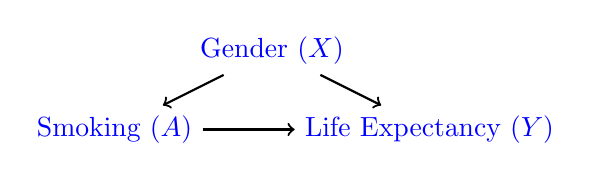
\begin{tikzpicture}[thick]
            \node (1) at (0,1) {\textcolor{Blue}{Gender ($ X $)}};
            \node (2) at (-2,0) {\textcolor{Blue}{Smoking ($ A $)}};
            \node (3) at (2,0) {\textcolor{Blue}{Life Expectancy ($ Y $)}};
            \draw[->] (1) to (2);
            \draw[->] (1) to (3);
            \draw[->] (2) to (3);
      \end{tikzpicture}
\end{figure}
\subsection*{Another Example of Confounding}
\begin{figure}[H]
      \centering
      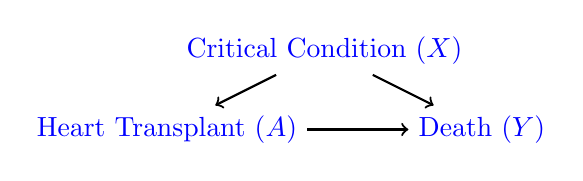
\begin{tikzpicture}[thick]
            \node (1) at (0,1) {\textcolor{Blue}{Critical Condition ($ X $)}};
            \node (2) at (-2,0) {\textcolor{Blue}{Heart Transplant ($ A $)}};
            \node (3) at (2,0) {\textcolor{Blue}{Death ($ Y $)}};
            \draw[->] (1) to (2);
            \draw[->] (1) to (3);
            \draw[->] (2) to (3);
      \end{tikzpicture}
\end{figure}
\subsection{Cross-sectional Studies}
\begin{itemize}
      \item Individuals are selected from the target population and their
            status with respect to the risk factor and the disease status is
            ascertained at the same time.
      \item The data represents a snapshot view of the relation between
            the risk factor and the event occurrence.
      \item Surveys are often cross-section in nature where associations
            are of interest and less priority is given to establishing
            causation.
      \item Advantage: cross-sectional studies are typically short.
      \item Disadvantage: a serious problem with such cross-sectional
            studies is the inability to determine whether the disease
            outcome or the risk factor occurred first, again this makes
            causal inferences more problematic or almost impossible.
\end{itemize}
\subsection{Cohort Studies}
\begin{itemize}
      \item Cohort studies typically include obtaining two groups from a
            pre-determined \# of individuals, one possessing and the other
            not possessing a risk factor of interest. Subsequent counts of
            cases (and non-cases) of a disease of interest are then
            recorded.
      \item Much more often than not, cohort studies are \textcolor{Red}{prospective}, but
            there are retrospective (or historical) cohort studies as well.
\end{itemize}
Table representing simple cohort study with sampling based on
risk-factor status:
\begin{table}[H]
      \centering
      \begin{NiceTabular}{|c|cc|c|}
            \toprule
            &\multicolumn{2}{c}{\emph{Disease}}\\
            \emph{Risk Factor} & Present ($ D $)                            & Absent ($ D^c $) & Total                                        \\
            \midrule
            Present ($ E $) & $ a $                            & $ b $                 & $ n_1 $         \\
            Absent ($ E^c $)  & $ c $                            & $ d $                 & $ n_2 $         \\
            \bottomrule
      \end{NiceTabular}
\end{table}
\begin{itemize}
      \item $ a \sim \BIN[\big]{n_1,\Prob{D\given E}} $.
      \item $ c \sim \BIN[\big]{n_2,\Prob{D\given E^c}} $.
\end{itemize}
\subsection{Case-control Studies}
\begin{itemize}
      \item In case-control studies, the direction of sampling differs from
            that of cohort studies. Specifically, the investigator selects a
            pre-determined \# of disease cases and non-cases (i.e.,
            controls), then looks retrospectively to see the \# of
            individuals with and without the risk factor in each group.
      \item Case-control studies are \textcolor{Red}{retrospective} studies.
\end{itemize}
Table representing simple case-control study with sampling based on
disease status:
\begin{table}[H]
      \centering
      \begin{NiceTabular}{|c|cc|}
            \toprule
            &\multicolumn{2}{c}{\emph{Disease}}\\
            \emph{Risk Factor} & Present                            & Absent                            \\
            \midrule
            Present & $ a $                            & $ b $             \\
            Absent   & $ c $                            & $ d $      \\
            \midrule
            Total & $ n_1 $ & $ n_2 $\\
            \bottomrule
      \end{NiceTabular}
\end{table}
\begin{itemize}
      \item $ a \sim \BIN[\big]{n_1,\Prob{E\given D}} $.
      \item $ b \sim \BIN[\big]{n_2,\Prob{E\given D^c}} $.
\end{itemize}